\chapter{Drupal} \label{Drupal}

\section{Wat is Drupal?}

\begin{wrapfigure}{r}{0.3\textwidth}
\vspace{-40pt}
%\hspace{-10pt}
\centering
\label{fig:drupalLogo}

\includegraphics[width=0.3\textwidth]{fig/drupalLogo}
\vspace{-30pt}
%\hspace{-10pt}
\centering
\caption{Drupallogo}
\centering
\vspace{-40pt}
\end{wrapfigure}
We kunnen Drupal het best beschrijven aan de hand van Figuur~\ref{fig:watIsDrupal}.
Drupal is een \textit{Content Management System} (CMS)\nomenclature{CMS}{Content Management System}, een \textit{framework} voor webapplicaties en een \textit{social publishing platform}. Maar Drupal is meer dan software alleen. Drupal staat voor een gemeenschap van ontwikkelaars en gebruikers met uiteenlopende doeleinden die elk hun eigen visie willen realiseren. \cite{drupalDefGuide}

\subsubsection{Content Management System}

Drupal levert alle functies en mogelijkheden van een krachtig CMS. We denken meteen aan het kunnen inloggen en registreren van gebruikers, verschillende soorten gebruikers kunnen defini\"{e}ren, verschillende niveaus van permissies,... Ook denken we aan het cre\"{e}ren, aanpassen, beheren, weergeven, categoriseren en aggregeren van content. Drupal biedt bovendien de mogelijkheid om modulair extra functionaliteit toe te voegen naar eigen noden en wensen.

\subsubsection{Framework voor webapplicaties}

Drupal is zeer flexibel en krachtig waardoor er enorm veel verschillende soorten webapplicaties mee kunnen gebouwd worden. Dit is deels te danken aan de API's die Drupal aanbiedt. Deze worden bij elke versie van Drupal uitgebreid maar ze worden niet complexer om te gebruiken. % Drupal's veelzijdigheid wordt nogmaals bewezen met het feit dat het zowel als frontend voor Java-gebaseerde applicaties kan optreden als voor backend voor AJAX of Flash-driven frontends.

\subsubsection{Social publishing platform}

Dat Drupal een social publishing platform is, houdt in dat content gemakkelijk te delen is via Drupal. Drupal biedt de mogelijkheid complexe data in een structuur te gieten die gemakkelijk uit te wisselen is. Op deze manier is het eenvoudig hetzelfde stuk content voor te stellen op verschillende websites.

\begin{figure}[h]
\centering
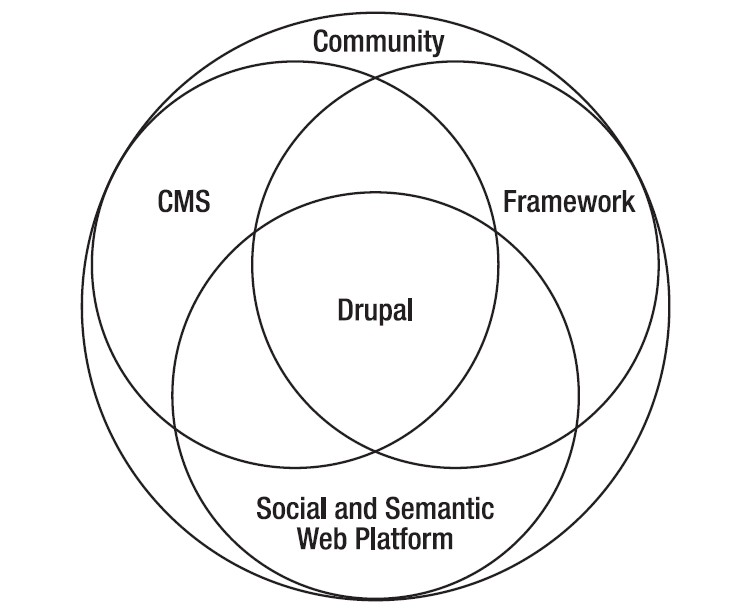
\includegraphics[width=0.4\textwidth]{fig/watIsDrupal}
\caption{Wat is Drupal?}
\vspace{-10pt}
\label{fig:watIsDrupal}
\end{figure}

We kunnen Drupal ook beschrijven als een gratis softwarepakket dat je de mogelijkheid biedt om jouw inhoud gebruiksvriendelijk te beheren en te publiceren. En dit op zo een manier dat je een eindeloze graad van personalisering hebt. Deze inhoud kan bestaan uit allerlei dingen, zoals: een blog, een video, een foto, een artikel, resultaten van een experiment,... Algemeen is dit dus een combinatie van tekst, beelden en audio die bezoekers van je website kunnen zien, lezen en/of horen. Bovendien is Drupal \textit{open source}.

Drupal is ontwikkeld in PHP en gebruikt ook een noemenswaardige hoeveelheid JavaScript (in de vorm van jQuery) voor de frontend. Voor het opslaan van content en configuratiegegevens gebruikt Drupal een relationele databank. Drupal in zijn huidige versie (7) kan op elk platform draaien onder volgende twee voorwaarden:
\begin{itemize}
\item Het platform bevat een webserver die PHP, en dus server-side scripting ondersteunt. Voorbeelden van deze webserver zijn:  Apache, IIS, Lighttpd en nginx.
\item Het platform ondersteunt een van volgende databanktechnologie\"{e}n: MySQL, SQLite of PostgreSQL.
\end{itemize}
Bij deze masterproef wordt er gebruik gemaakt van Apache en MySQL.

\subsection{Basiswebsite}

Wanneer je Drupal installeert beschik je meteen over een basiswebsite. Omdat je meteen al een bruikbare website hebt, is de drempel om Drupal te beginnen gebruiken dus laag. Deze website biedt meteen al een heleboel functionaliteit aan die geleverd wordt door de zogenaamde Drupal\textit{core}. %en een aantal out-of-the-boxfuncties.
\begin{figure}[h]
\begin{center}

\includegraphics[keepaspectratio,width=1\textwidth]{fig/drupalBasiswebsite}
\vspace{-10pt}
\caption{Basiswebsite van Drupal met Bartik-theme}
\vspace{-30pt}
\end{center}
\end{figure}

\section{Waarom Drupal?}

Eerst sommen we de vlakken op waar elke degelijke software goed op moet s\textit{core}n:
\begin{itemize}
\item betrouwbaarheid en robuustheid
\item effici\"{e}ntie
\item flexibiliteit
\end{itemize}
Als we dit even vergelijken met de principes waarop Drupal gebouwd is \cite{drupalMission}:
\begin{itemize}
\item Modulair en uitbreidbaar: Drupal kan uitgebreid worden met modules, waarbij je zelf ook modules kan ontwerpen indien er nog geen bestaat die aan jouw noden voldoet. Dit draagt dus bij aan de flexibiliteit.
\item Kwaliteitsvolle codering: kwaliteitsvolle, elegante en goed gedocumenteerde code is een prioriteit. Dit draagt bij tot de robuustheid en betrouwbaarheid.
\item \textit{Standard-based}: Drupal maakt gebruik van ingeburgerde standaarden zoals bijvoorbeeld XHTML en CSS. Dit draagt ook bij tot de robuustheid en betrouwbaarheid.
\item \textit{Low-resource demanding}: om een goede prestatie te garanderen, maakt Drupal gebruik van low-profile codering (bijvoorbeeld minimaliseren van databasequeries). Dit draagt bij tot de effici\"{e}ntie.
\item \textit{Open source}: Drupal is gebouwd op, en kan gebruikt worden in, andere \textit{open source}projecten.
\item Gebruiksvriendelijk: Drupal moet gemakkelijk te gebruiken zijn. Zowel voor gebruikers, ontwikkelaars en administrators van een website.
\item Samenwerking: Drupal voorziet systemen om samenwerking te bevorderen, waaronder het versiebeheersysteem GIT.
\end{itemize}
We zien dat Drupal aan de eerder vermelde voorwaarden voldoet.\\

\noindent
Een bijkomend voordeel van Drupal is zijn grote gemeenschap die ondertussen uit al meer dan 630000 actieve gebruikers en ontwerpers bestaat die zich dagelijks inspannen om Drupal steeds beter te maken. Dit aantal neemt elke dag toe. Dankzij die grote gemeenschap krijg je snel antwoord op je vragen door de medewerking van andere Drupalleden.\\

We bespreken nu enkele nadelen van Drupal:
\begin{itemize}
\item Aangezien Drupal gebruik maakt van een databank, heb je een databankserver nodig, al dan niet op dezelfde fysieke server als de webserver.
\item Bovendien wordt telkens een pagina wordt opgevraagd, de \textit{bootstrap}code uitgevoerd, waarbij ook nog eens de databank veelvuldig wordt geraadpleegd. 
Dit maakt Drupal relatief traag.
\item Drupal is zeer gebruiksvriendelijk en ideaal voor de eindgebruikers, die gemakkelijk en interactief inhoud willen toevoegen en beheren. 
Beginnende Drupalontwikkelaars zullen evenwel merken dat Drupal een erg steile leercurve heeft.
\item Ook ben je afhankelijk van de Drupalcommunity en dus de goodwill van de andere leden. Dit is in veel gevallen een voordeel, maar wanneer je een probleem hebt, ben je niet zeker of er wel een oplossing voor bestaat.
\item Tenslotte kan iedereen een module maken. Dit heeft natuurlijk zijn voordelen maar wanneer je een module van iemand anders gebruikt, ben je nooit zeker of de module zal onderhouden worden naar de toekomst toe en of er al dan niet bugs in zitten.
\end{itemize}

\section{Werking van Drupal}

Aan de hand van een voorbeeld \cite{drupalDefGuide} proberen we de lezer een idee te geven van de werking van Drupal. Bekijk Drupal als een digitale postzegelsorteerder. De nodes zijn de postzegels en de contenttypes zijn de verschillende soorten postzegels (postzegels van \euro~0,67, \euro~1,34, ... ). Naast contenttypes, kan je taxonomy gebruiken om een verdere onderverdeling te maken in de postzegels. De mate waarin en de criteria waarop je je onderverdeling maakt, kan je zelf kiezen (land, kleur, ...). Views is het mechanisme dat je postzegels sorteert en weergeeft in de vorm van pagina's en blocks. Van deze pagina's en blocks kan je zelf grootte, vorm, kleur en andere criteria opstellen zodat je deze helemaal kan personaliseren. Zie Figuur~\ref{fig:drupalGrafischeWeergave}.

\begin{figure}[h]
\centering
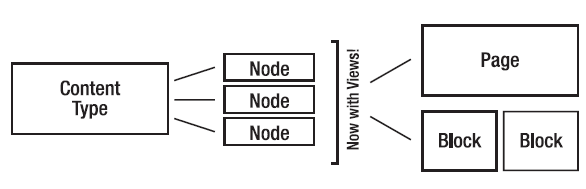
\includegraphics{fig/drupalGrafischeWeergave}
\centering
\vspace{-10pt}
\caption{Grafische weergave van hoe Drupal content aanbiedt.}
\vspace{-10pt}
\label{fig:drupalGrafischeWeergave}
\end{figure}

\subsection{Drupal bouwstenen}

We gaan dieper in op de begrippen die gebruikt worden in het voorbeeld en lichten enkele extra termen toe die ook gebruikt worden in Drupal.

\subsubsection{Content type}
Een contenttype bepaalt het soort content. Het bundelt soorten gegevens tot een logisch geheel. Wanneer content van een bepaald type wordt aangemaakt, worden de gegevens ingevuld door middel van \textit{Fields}. De toegevoegde content wordt een node genoemd. Ook biedt een contenttype de mogelijkheid om verschillende soorten content te onderscheiden van elkaar op basis van het type.
Drupal biedt gebruikers de mogelijkheid aan om hun eigen \textit{custom} contenttypes te maken.
%figuur van add contenttype

\subsubsection{Node}
Nodes zijn instanties van een contenttype. Een node kan maar aan \'{e}\'{e}n contenttype toebehoren.
Alle nodes hebben enkele eigenschappen gemeenschappelijk:
\begin{itemize}
\item Node id: zorgt voor een unieke identificatie.
\item Menu-instellingen: hier kan je een optionele menulink instellen zodanig dat je het menu op je website volledig kan personaliseren.
\item Mogelijkheden in verband met revisie: in de levensloop van de content kan je revisies maken zodat je terug kan keren naar een vorig moment indien er iets fout gaat met de content.
\item \textit{Uniform Resource Locator} (URL) \nomenclature{URL}{Uniform Resource Locator} pad instellingen: standaard is content beschikbaar via een URL van de vorm /node/node\_id. Maar via deze instellingen kan je een alias opgeven waarlangs de content ook (en dus gemakkelijker) beschikbaar is, dit principe heet in Drupal "\textit{Clean} URL's". De URL zal dan van de vorm /alias zijn.
\item Commentaarinstellingen: je kan zelf instellen of gebruikers commentaar kunnen achterlaten bij deze node.
\item Auteurinstellingen: hier stel je in of de creatietijd en auteur getoond moeten worden bij deze node.
\item Publicatieinstellingen: soms is het mogelijk dat je deze content nog niet beschikbaar wil stellen op de website, of je wil ze tijdelijk offline halen. Via deze instellingen is dit mogelijk.
\end{itemize}

\subsubsection{Fields}
Via \textit{Fields} kan je gegevens voor een contenttype invullen. Standaard biedt Drupal een aantal velden aan om gegevens toe te voegen, maar soms schieten deze velden tekort. Daarom heeft een gebruiker de mogelijkheid \textit{custom} velden te maken.

\subsubsection{View}
Views worden gebruikt om content visueel voor te stellen op welke manier dan ook. Een view is dan ook niet meer dan een visuele representatie van een verzameling content uit de datbank.

\subsubsection{Block}
Blocks zijn, zoals de naam al impliceert, blokken die een verzameling van herbruikbare content bevatten. Ze geven het beeld van die content. Blocks kunnen op gemakkelijke wijze toegevoegd worden aan je website waar jij dat wilt en hoe vaak je dat wilt. Het is bijvoorbeeld gemakkelijk om aan te geven dat je een bepaald block enkel op een bepaalde pagina wil laten verschijnen, en bovendien waar op de pagina je dat wilt. Merk echter wel op dat het hier niet echt content betreft, de inhoud van het block wordt aangemaakt bij opvraging en is dus geen blok beheerbare content. We zien een voorbeeld van een block in paragraaf \ref{jQuery}.

\subsubsection{Theme}
Themes zijn templates die bepalen hoe jouw website eruit ziet en aanvoelt voor de gebruiker. Net zoals modules zijn themes modulair en zijn ze dus gemakkelijk te wisselen, ook themes kunnen zelf ontwikkeld worden en zijn ter beschikking op de Drupal community.

\subsubsection{Taxonomy}
Taxonomy geeft je de mogelijkheid om eigenschappen en categorie\"{e}n toe te voegen aan je content, zodat bijvoorbeeld een gebruiker content kan filteren uit een grote verzameling. Het biedt dus een manier om je content te organiseren. Een praktijkvoorbeeld is een receptensite, een gebruiker kan dan recepten filteren aan de hand van de eigenschappen van het gerecht (ingredi\"{e}nten, moeilijkheid, ...).

\subsubsection{Gebruikers, rollen en permissies}
%Gebruikers zijn personen die zich aangemeld hebben op jouw website, met uitzondering van de anonieme gebruikers.
Alle gebruikerfunctionaliteit zoals registreren, inloggen, enz... zit reeds in de Drupal\textit{core}. Rollen geven weer tot welk type een gebruiker hoort. Meerdere gebruikers kunnen dezelfde rol hebben, en een gebruiker kan meerdere rollen hebben. Met permissies kan je aangeven welke privileges een gebruiker met een bepaalde rol heeft en dus wat die gebruiker mag en kan doen. Deze permissies worden gekoppeld aan een rol zodat alle gebruikers die deze rol hebben automatisch de privileges hebben van deze rol. Drupal biedt standaard drie rollen aan: de Administratorrol, die alle privileges bevat; de geauthenticeerde gebruikerrol, die een subset van de privileges van de Administratorrol bevat en de anonieme gebruikerrol, die een subset van de privileges van de geauthenticeerde gebruikerrol bevat. Anonieme gebruikers zijn gebruikers die zich niet aangemeld hebben op de website.

\subsubsection{Module}
Modules bieden de mogelijkheid om extra functionaliteit in te pluggen op een website. Modules zijn gratis te downloaden van de Drupal community en omdat deze community groot is, is de kans zeer groot dat er al een module gemaakt is voor jouw probleem. Indien dit niet het geval is, heb je nog altijd de mogelijkheid om zelf een module te ontwikkelen. Het gebruik van modules voorkomt ook dat functionaliteit die je niet nodig hebt, ook niet op jouw website komt. Je website is dus zeer configureerbaar naar eigen wensen (Zie figuur~\ref{fig:drupalOrganizeModules}).
\begin{figure}[h]
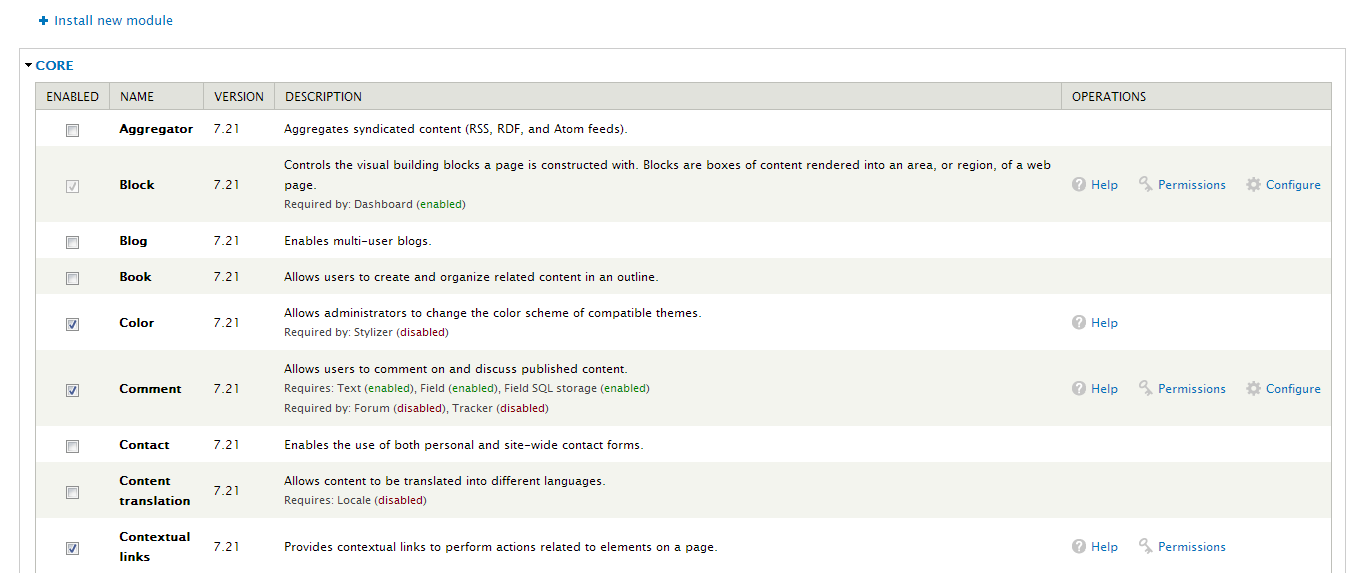
\includegraphics[width=1\textwidth]{fig/drupalOrganizeModules}
\caption{Organisatie van Drupalmodules}
\label{fig:drupalOrganizeModules}
\end{figure}

\subsubsection{Drupalcore}
De Drupal\textit{core} is wat je downloadt van de Drupalwebsite. Het vormt de basis en een uitgebreide \textit{out-of-the-box}functionaliteit, het fungeert eigenlijk als de motor achter een Drupalwebsite. De Drupal\textit{core} is zeer uitgebreid en complex, het vormt op zich al voldoende materiaal voor een scriptie, er verder op ingaan zou ons dus te ver leiden.

\subsubsection{Entities}
Een nieuw belangrijk concept in Drupal 7 is entities \cite{entities}. Dit nieuwe concept in combinatie met de Entity API heeft twee positieve effecten. Het eerste effect is dat gebruikers en commentaren dezelfde mogelijkheden krijgen als nodes. In vorige versies van Drupal was het niet mogelijk versies te cre\"{e}eren of velden toe te voegen aan gebruikers of commentaren. Andere voordelen zoals het gebruiken van views in combinatie met gebruikers of commentaren was ook niet mogelijk. Het andere effect is het invoeren van object-ge\"{o}rienteerd programmeren van entities. Vroeger was het nodig specifieke functies van de \textit{core} te gebruiken om content te bewerken. Een voorbeeld hier van is node\_save() dat nodes opslaat. Deze functie was enkel toepasbaar op een node. Het alternatief bij de Entity API is entity\_save(). Deze functie is niet gelimiteerd tot enkel content of enkel tot gebruikers.
Het is ook mogelijk nieuwe entities te maken. %, we gaan hier dieper op in in hoofdstuk~\ref{uitbreidingen}.

\subsubsection{Hooks}
Hooks zijn functies die gedefinieerd zijn door de Drupal\textit{core}. Ze kunnen worden ge\"{i}mplementeerd door elke module. In de Drupal\textit{bootstrap} zal de Drupal\textit{core} dan op bepaalde tijdstippen de bijhorende \textit{hooks} oproepen van elke module die de hook ge\"{i}mplementeerd heeft. Hiervoor wordt een zeer eenvoudig mechanisme gehanteerd. Een module kan zo'n hook defini\"{e}ren door de naam van de hook te laten voorafgaan door de naam van de module die de hook implementeert (zie codevoorbeeld~\ref{lst:drupalHookExample}).

\scriptsize
\lstset{language=PHP}
\begin{lstlisting}[label=lst:drupalHookExample,caption=Implementatie van hook\_node\_view door de module coap\_resource]
function coap_sensor_node_view($node, $view_mode, $langcode) {
  if($node->type == 'coap_resource'){
    _coap_resource_add_js();
  }
  else if($node->type == 'coap_device'){
    $node->content['coap_device_form'] = drupal_get_form('coap_device_form', $node);
  }
  return $node;
}
\end{lstlisting}
\normalsize

\subsection{Pagina aanroepen}
Elke keer een webbrowser een Drupal pagina opvraagt, gebeuren er een reeks complexe stappen die als eindresultaat de gerenderde pagina hebben. Indien de pagina niet aanwezig is in de cache, wordt de volledige \textit{bootstrap} en de \textit{page callback} uitgevoerd. De \textit{bootstrap} bestaat steeds uit dezelfde reeks van acht verschillende fasen die we verder nader toelichten. Na de \textit{bootstrap} wordt de \textit{page callback} uitgevoerd. Indien de pagina wel in de cache aanwezig is, wordt er enkel een subset van de stappen van de \textit{bootstrap} uitgevoerd. Het hele proces wordt weergegeven in Figuur~\ref{fig:drupalPageRendering}.

\begin{figure}
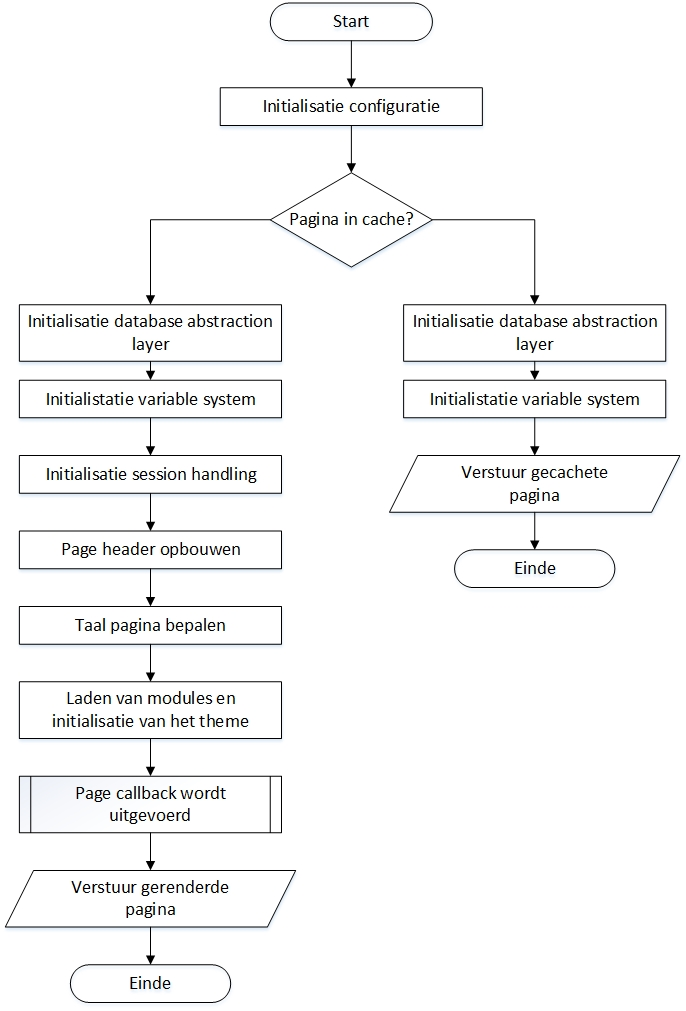
\includegraphics[width=1\textwidth]{fig/drupalPageRendering}
\caption{Pagina renderen in Drupal}
\label{fig:drupalPageRendering}
\end{figure}

\subsubsection{Initialisatie van de configuratie}
Deze fase houdt onder andere in dat globale variabelen worden gezet, zoals de basis-URL van de website. Deze configuratie gebeurt aan de hand van een configuratiebestand en aan de omgeving waarin de server zich bevindt.

\subsubsection{Poging tot opvragen van een gecachte pagina}
In deze fase tracht Drupal te vermijden dat de volledige \textit{bootstrap} moet worden doorlopen. Wanneer de pagina al eens is opgevraagd en deze nog geldig is, wordt ze uit de cache gehaald.

\subsubsection{Initialisatie van de database abstraction layer}
Basisklassen en functies worden ge\"{i}nitialiseerd, maar er worden nog geen verbindingen met de databank opgezet.

\subsubsection{Initialisatie van het Variable System}
In deze fase worden de waarden van variabelen uit de \textit{variable}tabel gehaald, die zich in de databank bevindt, en ingevuld bij de juiste naam. Als er modules zijn waarvan \textit{hooks} moeten worden opgeroepen, worden deze ook ingeladen.

\subsubsection{Initialisatie Session Handling}
In deze fase wordt aan elke user een sessie gekoppeld. Een anonieme user krijgt geen sessie toegewezen tenzij er iets in de sessie moet worden opgeslagen.

\subsubsection{Page Header opbouwen}
De eerste HTTP-\textit{headers} worden opgebouwd. Deze worden echter nog niet verstuurd, dit gebeurt pas op het einde van de cyclus. In deze fase vormt zich de eerste mogelijkheid voor modules om functionaliteit in te pluggen in de cyclus van de pagina.

\subsubsection{De taal van de pagina bepalen}
Als de website meerdere talen ondersteunt wordt in deze fase de gekozen taal van de gebruiker bepaald.

\subsubsection{Laden van modules en initialisatie van het theme}
Alle ingeschakelde modules worden ingeladen en het theme wordt ge\"{i}nitialiseerd. Deze fase biedt ook nog de mogelijkheid om variabelen in te stellen die pas later in de \textit{request} beschikbaar zijn.

\subsubsection{Uitvoeren van page callback}
Drupal bouwt en rendert de pagina.

\subsection{Database Abstraction Layer}
Manipulatie van gegevens in de databank gebeurt via de \textit{Database Abstraction Layer} \cite{databaseAbstractionLayer}. Dit zorgt ervoor dat de implemenatie van een module onafhankelijk is van de gebruikte soort databank. Concreet biedt deze laag een aantal functies aan voor het manipuleren van de databank. Wanneer een nieuw soort databank in gebruik genomen wordt, worden deze functies ge\"{i}mplementeerd voor deze nieuwe soort. We geven enkele voorbeelden van de meest gebruikte functies:
\lstset{language=PHP}
\begin{lstlisting}[label=db_select,caption=Voorbeeld gebruik van db\_select]
$result = db_select('coap_sensor_interested_user','resource')
	->fields('resource', array('nid'))
	->condition('uri', $uri, '=')
	->condition('uid', $user->uid, '=')
	->execute();
\end{lstlisting}
In voorbeeld \ref{db_select} wordt opgevraagd wat het nid is voor een specifieke uri en uid. Er wordt gebruik gemaakt van de Drupalvariabele \$user. Zoals je ziet moet er een naam opgegeven worden na de tabelnaam. Deze naam moet herhaalt worden als eerste element van de fieldstabel. Merk op dat dit alleen nodig is bij het gebruik van db\_select. Als tweede element van de fieldstabel geef je een tabel op met alle velden die je wil opvragen. Meerdere condities kunnen opgegeven worden, de volgorde is niet belangrijk. De opgevraagde gegevens kunnen gesorteerd worden door gebruik te maken van -\textgreater orderBy('nid', 'ASC').\\

De variabele \$result zal een \textit{SelectQuery}-object bevatten. Er zijn twee manieren om de opgehaalde gegevens uit objecten van deze klasse te halen. Wanneer je weet dat er maar een enkele rij opgehaald wordt, doe je best het volgende
\lstset{language=PHP}
\begin{lstlisting}
$record  = $result->fetchAssoc();
$nid = $record['nid'];
\end{lstlisting} 
Wanneer er meerdere rijen teruggegeven kunnen worden gebruik je beter
\lstset{language=PHP}
\begin{lstlisting}
$nids = array();
foreach($result as $record){
	$nids[] = $record->nid;
}
\end{lstlisting} 
om een tabel met al je gewenste resultaten in te bekomen. % In dit voorbeeld zal er echter maar \'{e}\'{e}n rij teruggegeven worden en is de eerste optie beter.
\lstset{language=PHP}
\begin{lstlisting}[label=db_insert,caption=Voorbeeld gebruik van db\_insert]
$id = db_insert('coap_sensor_interested_user')
	->fields(array(
		'uid' => $user->uid,
		'uri' => $resource_uri,
		'device' => 0,
		'nid' => $nid,
		'observe' => 0,
	))
	->execute();
\end{lstlisting}
In voorbeeld \ref{db_insert} wordt een entry toegevoegd aan de tabel coap\_sensor\_interested\_user. Kolommen die niet null mogen zijn en geen default waarde hebben moeten opgegeven worden in de fieldstabel. Zoniet wordt er een exceptie opgegooid bij het oproepen van de execute-functie.

\lstset{language=PHP}
\begin{lstlisting}[label=db_update,caption=Voorbeeld gebruik van db\_update]
$num_updated = db_update('coap_sensor_interested_user')
	->fields(array(
		'new' => 0,
	))
	->condition('uid', $user->uid, '=')
	->condition('device',1,'=')
	->condition('nid', $nid, '=')
	->execute();
\end{lstlisting}
In voorbeeld \ref{db_update} wordt van alle rijen die overeenstemmen met de opgegeven condities de new-waarde op 0 gezet. % Bij dit voorbeeld zal er maar \'{e}\'{e}n rij geupdated worden.

\lstset{language=PHP}
\begin{lstlisting}[label=db_delete,caption=Voorbeeld gebruik van db\_delete]
db_delete('coap_sensor_interested_user')
	->condition('nid', $nid, '=')
	->execute();
\end{lstlisting}
In voorbeeld \ref{db_delete} worden alle rijen met als nid de waarde in \$nid verwijderd. % Opnieuw zal in dit voorbeeld maar \'{e}\'{e}n rij verwijderd worden.

\subsection{Installatie contenttypes}
Voor we uitleggen hoe de contenttypes ge\"{i}nstalleerd en gede\"{i}nstalleerd worden, merken we op dat er naast de\"{i}nstalleren van een module ook \textit{disablen} mogelijk is. Dit kan als gevolg hebben dat een beginnende Drupalontwikkelaar enkele dingen over het hoofd ziet. We maken een opsomming van handige feiten in verband met \textit{enablen}, \textit{disablen} en de\"{i}nstalleren voor beginnende Drupalontwikkelaars:
\begin{itemize}
\item Bij \textit{disablen} wordt hook\_disable() opgeroepen. Dit is analoog voor \textit{enablen}, installeren en de\"{i}nstalleren.
\item Een gebruiker moet een module altijd eerst \textit{disablen} voor te de\"{i}nstalleren.
\item Een gebruiker kan een module enkel \textit{enablen}, \textit{disablen} of de\"{i}nstalleren. Een module wordt ge\"{i}nstalleerd als ze voor de eerste keer enabled wordt of eerst gede\"{i}nstalleerd werd voor te \textit{re-enablen}.
\item Sommige \textit{hooks} worden maar opgeroepen bij installatie van de module, wat betekent dat wanneer je een wijziging van deze \textit{hooks} wil doorvoeren, je de module moet \textit{disablen}, de\"{i}nstalleren en \textit{re-enablen}. De\"{i}nstallatie mag niet worden overgeslagen omdat de module dan niet geherinstalleerd wordt. Dit is van toepassing bij volgende \textit{hooks}:
\begin{itemize}
\item hook\_node\_info()
\item hook\_schema()
\end{itemize}
\end{itemize}

\noindent
Er zijn meerdere manieren om contenttypes te installeren en configureren.
\begin{itemize}
\item De functie node\_type\_save() gebruiken om een nieuw type zelf op te slaan.
\item Hook\_node\_info() gebruiken waarin je de nieuwe contenttypes beschrijft. Deze optie wordt algemeen als de betere optie gezien omdat het gebruik van \textit{hooks} de\textit{ Drupal way} is.
\end{itemize}
Bij zowel de eerste als de tweede optie zijn nog een zaken nodig om een contenttype te configureren. Een aantal rijen moeten toegevoegd worden in de \textit{variable}tabel die standaard ge\"{i}nstalleerd wordt door Drupal. Deze speciale tabel heeft maar twee kolommen, \textit{name} en \textit{value}. Deze tabel wordt gemanipuleerd met speciale functies:
\begin{itemize}
\item variable\_get(\$naam): De variabele wordt opgehaald. Een tweede parameter kan opgegeven worden, als de variabele niet in de databank zit wordt deze waarde teruggegeven en wordt de variabele toegevoegd in de databank.
\item variable\_set(\$naam, \$value): De variabele wordt gezet.
\item variable\_del(\$naam): De variabele wordt verwijderd.
\end{itemize}

\noindent
In hook\_enable() worden enkele variabelen gezet. Deze variabelen moeten voor elk contenttype gezet worden. We degenen op die we gebruiken:
\begin{itemize}
\item comment\_content\_type: Krijgt de waarde 0 om default commentaren uit te schakelen.
\item node\_options\_content\_type: Krijgt de waarde array('status') om default '\textit{Promote to Front page}' uit te vinken.
\item node\_preview\_content\_type: Krijgt de waarde 0 om de mogelijkheid tot een preview te \textit{disablen}.
\item node\_submitted\_content\_type: Krijgt de waarde 1 om default de auteur en de tijd waarop de content is toegevoegd te tonen bij de content zelf.
\end{itemize}
Welke opties beschikbaar zijn vind je hier \cite{contentTypeVariables}.\\

\noindent
De laatste stap bestaat uit het cre\"{e}eren van de velden die toegevoegd gaan worden aan de contenttypes, vervolgens worden er instanties van de velden aangemaakt om ze te linken aan de contenttypes. Dit gebeurt in hook\_install(). De velden worden aangemaakt field\_create\_field(\$field) en de instanties worden aangemaakt met field\_create\_instance(\$instance). Er worden velden aangemaakt voor: de URI van devices, de URI van resources, meerdere referenties naar content van het type coap\_resource. %misschien moet dit wat uitgebreider

\subsection{De\"{i}nstallatie contenttypes}
De contenttypes worden verwijderd in hook\_uninstall(). Voor een contenttype kan verwijderd worden moet nog een aantal andere zaken verwijderd worden. We overlopen de verschillende stappen die voor elk te verwijderen contenttype moeten overlopen worden:
\begin{itemize}
\item Alle content van het contenttype wordt verwijderd door middel van de functie node\_delete\_multiple(\$nids). De variabele \$nid bevat een array met alle nids van de content die verwijderd wordt.
\item Alle variabelen die toegevoegd werden in de \textit{variable}tabel worden verwijderd door gebruik te maken van variable\_del(\$naam);
\item De commententiteit die geassocieerd is met dit contenttype wordt gemarkeerd om te verwijderen. Hiervoor wordt de functie field\_delete\_instance() gebruikt.
\item Het contenttype wordt verwijderd met node\_type\_delete(\$type\_name).
\item De databankcache van node types wordt geupdated met node\_types\_rebuild(). Dit is nodig omdat Drupal vaak in caches kijkt en verouderde informatie kan gebruiken.
\item Drupal zal bij het verwijderen van velden de kolomwaarde deleted op 1 zetten. Om de velden effectief uit de databank te verwijderen wordt de functie field\_purge\_batch() gebruikt.
\end{itemize}

\section{JQuery in Drupal} \label{jQuery}

\begin{wrapfigure}{r}{0.25\textwidth}
\vspace{-40pt}
\hspace{-10pt}
\centering
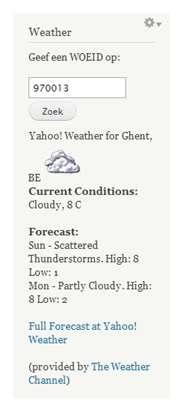
\includegraphics[width=0.3\textwidth]{fig/weermodule}
\vspace{-30pt}
\hspace{-10pt}
\centering
\caption{Weermodule}
\label{fig:weermodule}
%\centering
\vspace{-70pt}
\end{wrapfigure}

In deze paragraaf bekijken we hoe een module (weather\_info) gemaakt werd die het weerbericht ophaalt voor een regio naar keuze, aangegeven door een WOEID. In eerste instantie werd gewerkt met een formulier, maar in een latere fase werd overgestapt op jQuery, wat de gebruikerservaring bevordert.

\subsection{Met een formulier}

In eerste instantie bevatte de module een formulier bestaande uit een tekstveld als invoer voor de WOEID en een knop om het formulier in te dienen.
Wanneer de gebruiker op de knop klikt, gebeuren volgende stappen:

\begin{itemize}
	\item het formulier wordt ingediend
	\item de pagina wordt opnieuw geladen
	\item de \textit{bootstrap}code roept hook\_form\_submit() op door weather\_location\_form\_submit() op te roepen (weather\_location is de naam van het formulier):
	\begin{itemize}
		\item het ingegeven WOEID wordt opgeslagen op serverniveau met de Drupalfunctie variable\_set()
	\end{itemize}
	\item de \textit{bootstrap}code roept hook\_block\_view op van de weermodule door weather\_info\_block\_view() op te roepen:
	\begin{itemize}
		\item het ingegeven WOEID wordt opgehaald met behulp van de Drupalfunctie variable\_get()
		\item er wordt een HTTP-\textit{request} uitgevoerd naar de \textit{Yahoo Weather API} met de PHP-functie file\_get\_contents(), dat een URL als parameter verwacht
		\item het ontvangen xml-bestand wordt in een object gestopt met de PHP-functie SimplexmlElement(), waarna het weerbericht gemakkelijk uit het XML-bestand kan gehaald worden
		\item Het weerbericht wordt toegevoegd aan de inhoud van het block
	\end{itemize}
	\item De pagina wordt in de browser weergegeven met het weerbericht in het block
\end{itemize}

\subsection{Met AJAX in jQuery}

Een pagina zal pas getoond worden wanneer de \textit{bootstrap} afgelopen is en aangezien de code in de \textit{hooks} die worden uitgevoerd onderdeel is van de \textit{bootstrap}, zal de pagina pas getoond worden wanneer de \textit{hooks} afgelopen zijn. Dit heeft als gevolg dat de gebruiker van de website langer moet wachten op de pagina omdat eerst nog een HTTP-\textit{request} moet gebeuren om het weerbericht op te halen. Het spreekt voor zich dat dit een zeer nadelig effect is dat moet vermeden worden.\\
Als alternatief hebben we gekozen om een jQuery-event te koppelen aan de submit-knop die het formulier indient. jQuery is namelijk geschreven in JavaScript en JavaScript is een \textit{client-side scripting language}, wat inhoudt dat deze code wordt uitgevoerd op de machine van de gebruiker en dit nadat de pagina geladen is.\\
Wanneer de gebruiker op de knop klikt, wordt een \textit{Asynchronous JavaScript and XML}(AJAX)-\textit{call}\nomenclature{AJAX}{Asynchronous JavaScript and XML} uitgevoerd.
Zoals de naam suggereert, is dit een asynchrone aanroep, wanneer het antwoord aankomt wordt automatisch een opgegeven functie opgeroepen waarin de data kan verwerkt worden. Als gevolg heeft de gebruiker dus geen enkele hinder van het internetverkeer dat noodzakelijk is om het weerbericht op te halen.


\subsection{Problemen}

JQuery laat geen \textit{cross-domain} AJAX \textit{calls} toe wegens veiligheidsoverwegingen. Een oplossing hiervoor is een \textit{proxy}script in PHP gebruiken.
De AJAX-\textit{call} gebeurt dan naar het \textit{proxy}script dat zich op de server en dus hetzelfde domein bevindt. Het \textit{proxy}script vraagt daar effectief de data op en geeft de uitvoer terug.
De browser wordt dus eigenlijk om de tuin geleid. \cite{crossDomainProblem}
